\documentclass[svgnames]{beamer}

\usepackage{pri}
\usepackage{alltt}
\usepackage{graphicx}
\usepackage{tikz}
\usepackage{listings}

\graphicspath{{./}{figures/}{figures/08-xml-figs/}} 

\subtitle{Semi-Structured Data : JSON , XML and XPath}

\begin{document}

\maketitle

\begin{frame} \frametitle{Bibliography}

   \begin{block}{}
        \href{http://www.cs.uic.edu/~liub/WebMiningBook.html}{Bing Liu, Web Data Mining: Exploring Hyperlinks, Contents, and
         Usage Data, 2nd edition}. Chapter 9.
    \end{block}

   \begin{block}{}

    \href{http://www.mir2ed.org/}{Ricardo Baeza-Yates,
            Berthier Ribeiro-Neto, Modern Information Retrieval, 2nd
            edtion}. Chapter 13.

    \end{block}

   \begin{block}{}

    \href{http://nlp.stanford.edu/IR-book/}{Christopher D. Manning, Prabhakar Raghavan and Hinrich Schütze, Introduction to Information Retrieval.} Chapter 10.

    \end{block}
    
\end{frame}

\begin{frame}
\frametitle{Some Additional References}

\begin{itemize}
 \item XML Files website {\scriptsize (\url{http://www.xmlfiles.com})} \\
 {\it by Jan Egil Refsnes}
 \item XML in a  Nutshell {\scriptsize (\url{http://www.cafeconleche.org/books/xian3/})} \\
 {\it by Elliotte Rusty Harold; W. Scott Means}
 \item XML Tutorial {\scriptsize (\url{http://www.w3schools.com/xml/default.asp})} \\
 {\it by w3schools}
 \item Introducing JSON {\scriptsize (\url{http://www.json.org})} 
\end{itemize}

\end{frame}

\section{Semi-Structured Data}

%------------------------------------------------

\begin{frame}
\frametitle{Unstructured versus Structured Data}

\begin{block}{}
Traditionally, IR systems deal with information from unstructured text - by which we mean {\it raw} text without markup
\end{block}

\begin{block}{}
Traditionally, data management technology focuses on tabular data (i.e., relational model or field-delimited files)
\end{block}

\begin{center}
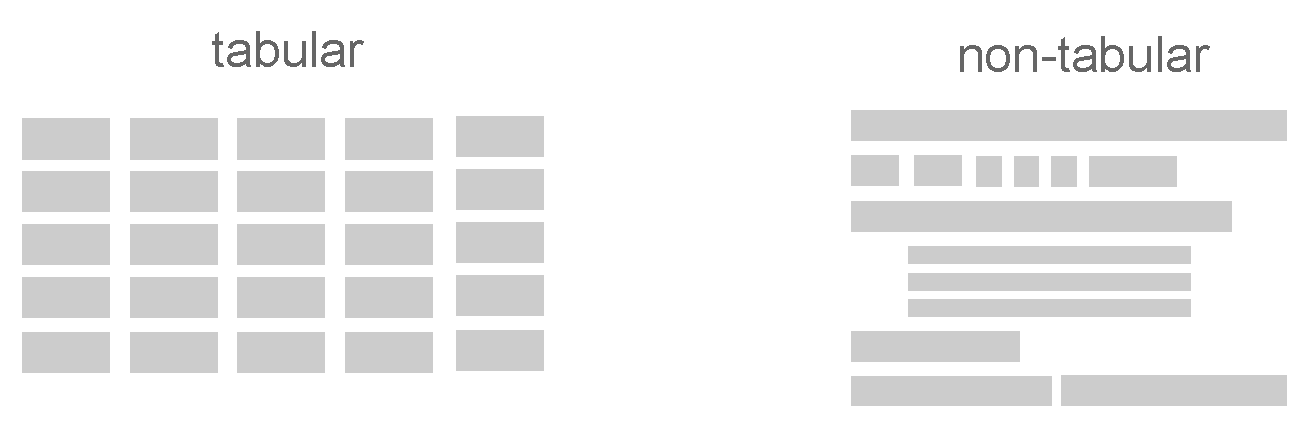
\includegraphics[width=10cm]{tabular_nontabular.pdf}
\end{center}

\end{frame}

%------------------------------------------------

\begin{frame}
\frametitle{Motivation}

\begin{block}{}
Many structured data sources containing text are best modeled as structured documents rather than  relational data
\end{block}

\begin{block}{}
Important limitations:
\begin{itemize}
  \item Compromise between {\it free text} and rigid data schemas
  \item In plain text formats there is no information to describe the location of the data values
  \item No recognizable label for each data value within the file
  \item Serious limitations to store data with hierarchical structure 
  \item We would like to support querying with basis on textual content, data values, and structural restrictions
\end{itemize}
\end{block}

\begin{block}{}
\begin{center}
\emph{Semi-structured data = Trees with text at leaves}
\end{center}
\end{block}

\end{frame}

%------------------------------------------------

\begin{frame}
\frametitle{Hierarchical data}
\begin{center}
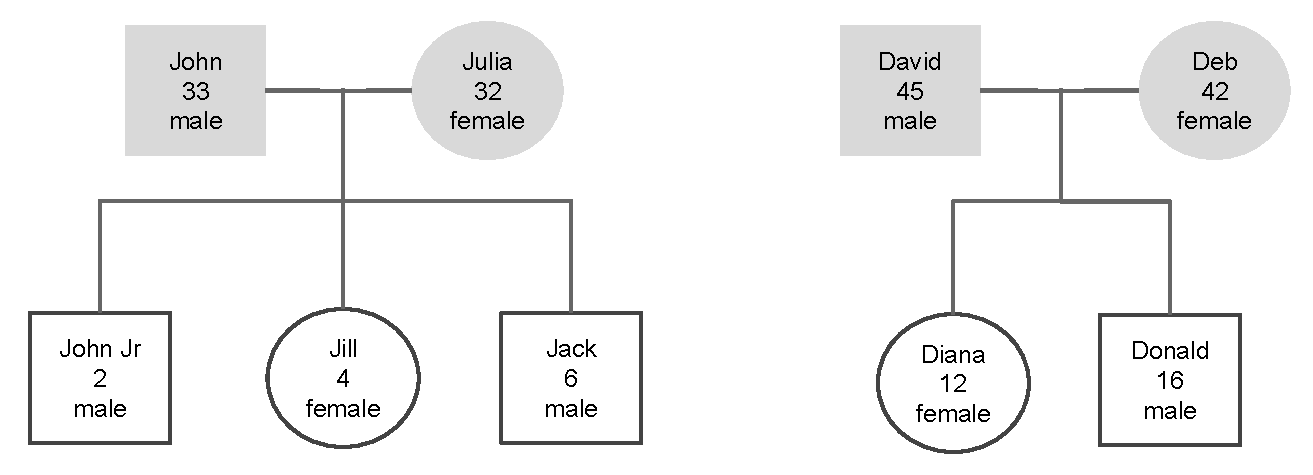
\includegraphics[width=10cm]{hierarchical_data.pdf}
\end{center}
\end{frame}

%------------------------------------------------

\begin{frame}[fragile]
\frametitle{Hierarchical data}

Field-delimited files have limitations with hierarchical data
\bigskip

\begin{verbatim}
                   John      33  male
                   Julia     32  female
    John   Julia   Jack       6  male
    John   Julia   Jill       4  female
    John   Julia   John jnr   2  male
                   David     45  male
                   Debbie    42  female
    David  Debbie  Donald    16  male
    David  Debbie  Dianne    12  female
\end{verbatim}

\end{frame}

%------------------------------------------------

\begin{frame}
\frametitle{XML and JSON formats}

XML - eXtensible Markup Language
\begin{itemize}
  \item XML is a data format that is still based on plain text
  \item Flexibility in terms of the schema for the data (e.g., a \emph{meta-language} that provides structure and syntax for representing any type of information -- not its semantics)
  \item In XML every single value is distinctly labeled, and every single value is self-described
  \item The information is organized hierarchically, in a much more sophisticated manner than with field-delimited files 
\end{itemize}

~\\

JSON - JavaScript Object Notation
\begin{itemize}
\item Simpler and less verbose than XML
\end{itemize}

\end{frame}

%------------------------------------------------

\begin{frame}[fragile]
\frametitle{Semi-Structured Data (1)}

An example of hierarchical data in XML
\begin{knitrout}\footnotesize
\definecolor{shadecolor}{rgb}{0.969, 0.969, 0.969}\color{fgcolor}\begin{kframe}
\begin{alltt}
<families>
 <family>
  <parent gender=\hlstr{"male"} name=\hlstr{"John"} age=\hlstr{"33"} />
  <parent gender=\hlstr{"female"} name=\hlstr{"Julia"} age=\hlstr{"32"} />
  <child gender=\hlstr{"male"} name=\hlstr{"Jack"} age=\hlstr{"6"} />
  <child gender=\hlstr{"female"} name=\hlstr{"Jill"} age=\hlstr{"4"} />
  <child gender=\hlstr{"male"} name=\hlstr{"John jnr"} age=\hlstr{"2"} />
 </family>
 <family>
  <parent gender=\hlstr{"male"} name=\hlstr{"David"} age=\hlstr{"45"} />
  <parent gender=\hlstr{"female"} name=\hlstr{"Debbie"} age=\hlstr{"42"} />
  <child gender=\hlstr{"male"} name=\hlstr{"Donald"} age=\hlstr{"16"} />
  <child gender=\hlstr{"female"} name=\hlstr{"Dianne"} age=\hlstr{"12"} />
 </family>
</families>
\end{alltt}
\end{kframe}
\end{knitrout}

\end{frame}

\begin{frame}[fragile]
\frametitle{Semi-Structured Data (2)}

An example of hierarchical data in JSON
\begin{knitrout}\scriptsize
\definecolor{shadecolor}{rgb}{0.969, 0.969, 0.969}\color{fgcolor}\begin{kframe}
\begin{alltt}
\{
 "families": [
    \{
	      "parents" : [
        \{ "gender": "male", "name": "John", "age": "33" \},
        \{ "gender": "female", "name": "Julia", "age": "32" \} ],
	      "childs": [
	        \{ "gender": "male", "name": "Jack", "age": "6" \},
        \{ "gender": "female", "name": "Jill", "age": "4" \},	
        \{ "gender": "male", "name": "John jnr", "age": "2" \} ]
    \} , \{  
	      "parents" : [
        \{ "gender": "male", "name": "David", "age": "45" \},
        \{ "gender": "female", "name": "Debbie", "age": "42" \} ],
	      "childs": [
	        \{ "gender": "male", "name": "Donald", "age": "16" \},
        \{ "gender": "female", "name": "Dianna", "age": "12" \} ]
    \}
  ]
\}
\end{alltt}
\end{kframe}
\end{knitrout}
\end{frame}

%------------------------------------------------

\begin{frame}
\frametitle{XML and HTML}

Why should you care about JSON, XML and HTML?
\begin{itemize}
  \item Large amounts of data and information are stored, shared and distributed using HTML, JSON and XML dialects
  \item Widely adopted and used in many applications
  \item Working with data from the Web means dealing with HTML (and JSON data comming from Web APIs)
\end{itemize}

\end{frame}

\section{JavaScript Object Notation}

\begin{frame}
\frametitle{JavaScript Object Notation (JSON)}

It is a fairly simple, lightweight method of representing data
\begin{itemize}
  \item Its origins lay in the JavaScript language, but JSON is language independent and text-based
  \item JSON is self-describing and easy to understand
  \item Format is syntactically identical to the code for creating JavaScript objects
\end{itemize}

\end{frame}


\begin{frame}
\frametitle{JSON Syntax}

JSON syntax is derived from JavaScript object notation syntax:
\begin{itemize}
  \item Data is in objects consisting of name/value pairs
  \item Data is separated by commas
  \item Curly braces hold data objects
  \item Square brackets hold arrays
\end{itemize}

~\\
A JavaScript program can use standard JavaScript functions to convert JSON data into native JavaScript objects

\begin{itemize}
\item You can search a JSON tree with jQuery
\item In Python, you can encode/decode basic object hierarchies
\item ...
\end{itemize}

\end{frame}



\begin{frame}
\frametitle{JSON Values}

JSON values can be:
\begin{itemize}
  \item Primitive types
    \begin{itemize}
    \item A number (integer or floating point)
    \item A string (in double quotes)
    \item A Boolean (true or false)
    \item Null - the {\it empty object}
    \end{itemize}
  \item Nested containers (i.e., containers can contain other containers or scalar values)
  \begin{itemize}
    \item An array (in square brackets)
    \item An object (in curly braces)
  \end{itemize}
\end{itemize}
\end{frame}

\begin{frame}[fragile]
\frametitle{Some Examples}
\begin{block}{JSON Objects}
\begin{verbatim}
{ "firstName":"John", "lastName":"Doe" }
\end{verbatim}
\end{block}

\bigskip

\begin{block}{JSON Arrays}
\begin{verbatim}
{"employees":[
    {"firstName":"John", "lastName":"Doe"},
    {"firstName":"Anna", "lastName":"Smith"},
    {"firstName":"Peter", "lastName":"Jones"}
] }
\end{verbatim}
\end{block}

\end{frame}

%------------------------------------------------

\section{eXtensible Markup Language}

%------------------------------------------------

\begin{frame}
\frametitle{Some Definitions}

\begin{quotation}
``XML is a markup language that defines a set of rules for encoding documents in a format that is both human-readable and machine-readable''
\end{quotation}

{\footnotesize 
\hspace{8mm} \url{http://en.wikipedia.org/wiki/XML}
}

\bigskip
\begin{quotation}
``XML is a data description language used for describing data''
\end{quotation}

{\footnotesize 
\hspace{8mm} {\hilit Paul Murrell} \\
\hspace{8mm} {\lolit Introduction to Data Technologies}
}

\end{frame}

%------------------------------------------------

\begin{frame}
\frametitle{Some Definitions}

\begin{quotation}
``XML is a very general structure with which we can define any number of new formats to represent arbitrary data''
\end{quotation}

\begin{quotation}
``XML is a standard for the semantic, hierarchical representation of data''
\end{quotation}

{\footnotesize 
\hspace{8mm} {\hilit Deb Nolan \& Duncan Temple Lang} \\
\hspace{8mm} {\lolit XML and Web Technologies for Data Sciences with R}
}

\end{frame}

%------------------------------------------------

\begin{frame}
\frametitle{About XML}

\begin{block}{XML}
XML stands for \emph{eXtensible Markup Language}
\end{block}

\begin{block}{Broadly speaking ...}
XML provides a flexible framework to create formats for describing and representing data
\end{block}

\end{frame}

%------------------------------------------------

\begin{frame}
\frametitle{Markup Languages}

\begin{block}{Markup}
A \emph{markup} is a sequence of characters or other symbols inserted at certain places in a document to indicate either: 
\begin{itemize}
 \item How the content should be displayed when printed or in screen
 \item To describe the document's structure
\end{itemize}
\end{block}

\begin{block}{Markup Language}
A markup language is a system for \emph{annotating} (i.e. \textit{marking}) a document in a way that the content is distinguished from its representation (e.g., LaTeX, PostScript, HTML, SVG)
\end{block}

\end{frame}

%------------------------------------------------

\begin{frame}[fragile]
\frametitle{XML Markups}

\begin{block}{XML Markups}
In XML (as well as in HTML) the marks (aka \textit{tags}) are defined using angle brackets: {\Large {\hilit \code{<>}}}
\end{block}

\bigskip

\code{{\hilit <mark>}Text marked with special tag{\hilit </mark>} }

\end{frame}

%------------------------------------------------

\begin{frame}[fragile]
\frametitle{XML is Extensible}

\begin{block}{XML is Extensible}
The concept of \textit{extensibility} means that we can define our own marks, the order in which they occur, and how they should be processed. For example:

~\\

 \begin{itemize}
  \item \code{<my\_mark>}
  \item \code{<awesome>}
  \item \code{<boring>}
  \item \code{<cool>}
 \end{itemize}
~\\

By defining marks, we give \emph{semantics} to the data.
\end{block}

\end{frame}

%------------------------------------------------

\begin{frame}
\frametitle{About XML}

\begin{block}{XML is NOT}
\begin{itemize}
 \item A programming language
 \item A network transfer protocol
 \item A database
 \item A representation format that encodes data semantics
\end{itemize}
\end{block}

\begin{block}{XML is}
\begin{itemize}
 \item A markup language ({\it although the term can refer to more than just that})
 \item A generic language that provides structure and syntax for representing any type of information
 \item A meta-language: it allows us to create or define other languages
\end{itemize}
\end{block}

\end{frame}

%------------------------------------------------

\begin{frame}
\frametitle{XML Applications}

\begin{block}{Some XML dialects}
\begin{itemize}
  \item \textbf{(X)HTML} (\textit{HyperText Markup Language}) for describing content in Web pages
 \item \textbf{KML} (\textit{Keyhole Markup Language}) for describing geo-spatial information used in Google Earth, Google Maps, Google Sky
 \item \textbf{SVG} (\textit{Scalable Vector Graphics}) for visual graphical displays of two-dimensional graphics with support for interactivity and animation
 \item \textbf{PMML} (\textit{Predictive Model Markup Language}) for describing and exchanging models produced by data mining and machine learning algorithms
\end{itemize}
\end{block}

\end{frame}

%------------------------------------------------

\begin{frame}[fragile]
\frametitle{Keyhole Markup Language - An Example}

\begin{knitrout}\footnotesize
\definecolor{shadecolor}{rgb}{0.969, 0.969, 0.969}\color{fgcolor}\begin{kframe}
\begin{alltt}
<kml xmlns=\hlstr{"http://www.opengis.net/kml/2.2"}>
<Document>
<Placemark>
  <name>New York City</name>
  <description>New York City</description>
  <Point>
    <coordinates>-74.006393,40.714172,0</coordinates>
  </Point>
</Placemark>
</Document>
</kml>
\end{alltt}
\end{kframe}
\end{knitrout}

\end{frame}

%------------------------------------------------

\begin{frame}[fragile]
\frametitle{Scalable Vector Graphics - Two Examples}

\begin{knitrout}\scriptsize
\definecolor{shadecolor}{rgb}{0.969, 0.969, 0.969}\color{fgcolor}\begin{kframe}
\begin{alltt}
<svg width=\hlstr{"100"} height=\hlstr{"100"}>
  <circle cx=\hlstr{"50"} cy=\hlstr{"50"} r=\hlstr{"40"} stroke=\hlstr{"green"} stroke-width=\hlstr{"4"} />
</svg>
  
  
<svg width=\hlstr{"400"} height=\hlstr{"110"}>
  <rect width=\hlstr{"300"} height=\hlstr{"100"} style=\hlstr{"fill:\hlkwd{rgb}(0,0,255)"} />
</svg>
\end{alltt}
\end{kframe}
\end{knitrout}

\end{frame}

%------------------------------------------------

\begin{frame}[fragile]
\frametitle{XML Example}

\begin{center}

\includegraphics[width=4cm]{goodwillhunting.jpg}
\end{center}
\begin{block}{Ultra Simple XML}
{\Large \begin{verbatim}
<movie>
  Good Will Hunting
</movie>
\end{verbatim}
}
\end{block}

\end{frame}

%------------------------------------------------

\begin{frame}[fragile]
\frametitle{XML Example}

\begin{block}{Ultra Simple XML}
\begin{verbatim}
<movie>
  Good Will Hunting
</movie>
\end{verbatim}
\end{block}

\bigskip

\begin{itemize}
 \item one single element {\textit{movie}}
 \item start-tag: {\hilit \code{<movie>}}
 \item end-tag: {\hilit \code{</movie>}}
 \item content: \code{Good Will Hunting}
\end{itemize}

\end{frame}

%------------------------------------------------

\begin{frame}[fragile]
\frametitle{XML Example}

\begin{block}{Ultra Simple XML}
\begin{verbatim}
<movie mins="126" lang="en">
  Good Will Hunting
</movie>
\end{verbatim}
\end{block}

\bigskip

\begin{itemize}
 \item XML elements can have \textbf{attributes}
 \item Attributes:  \code{\hilit mins} (minutes) and \code{\hilit lang} (language)
 \item Attributes are \textit{attached} to the element's start tag
 \item Attribute values \emph{must be quoted}
 \item Attributes are \emph{not ordered}
\end{itemize}

\end{frame}

%------------------------------------------------

\begin{frame}[fragile]
\frametitle{XML Example}

\begin{block}{Minimalist XML}
\begin{verbatim}
<movie mins="126" lang="en">
  <title>Good Will Hunting</title>
  <director>Gus Van Sant</director>
  <year>1998</year>
  <genre>drama</genre>
</movie>
\end{verbatim}
\end{block}

\bigskip

\begin{itemize}
 \item An XML element may contain other elements
 \item Element \textit{movie} contains several elements: \textit{title, director, year, genre}
 \item Child elements are ordered
\end{itemize}

\end{frame}

%------------------------------------------------

\begin{frame}[fragile]
\frametitle{XML Example}

\begin{block}{Simple XML}
\begin{verbatim}
<movie mins="126" lang="en">
  <title>Good Will Hunting</title>
  <director>
    <first_name>Gus</first_name>
    <last_name>Van Sant</last_name>
  </director>
  <year>1998</year>
  <genre>drama</genre>
</movie>
\end{verbatim}
\end{block}

\bigskip

\begin{itemize}
 \item Nested structures : now \textit{director} has two child elements: \textit{first\_name} and \textit{last\_name}
\end{itemize}

\end{frame}

%------------------------------------------------

\begin{frame}[fragile]
\frametitle{XML Hierarchy Structure}

\begin{block}{Conceptual XML}
\scriptsize
\begin{verbatim}
<Root>
  <child_1>...</child_1>
  <child_2>...</child_2>
    <subchild>...</subchild>
  <child_3>...</child_3>
</Root>
\end{verbatim}
\end{block}

\begin{itemize}
 \item An XML document can be represented with as a \emph{tree}
 \item An XML document must have \emph{one single root} element
 \item The \code{root} may contain \code{child} elements
 \item A \code{child} element may contain \code{subchild} elements
\end{itemize}

\begin{block}{Traversing the tree}
There's a \emph{unique} path from the root node to any given node 
\end{block}

\end{frame}

%------------------------------------------------

\begin{frame}
\frametitle{}
\begin{center}
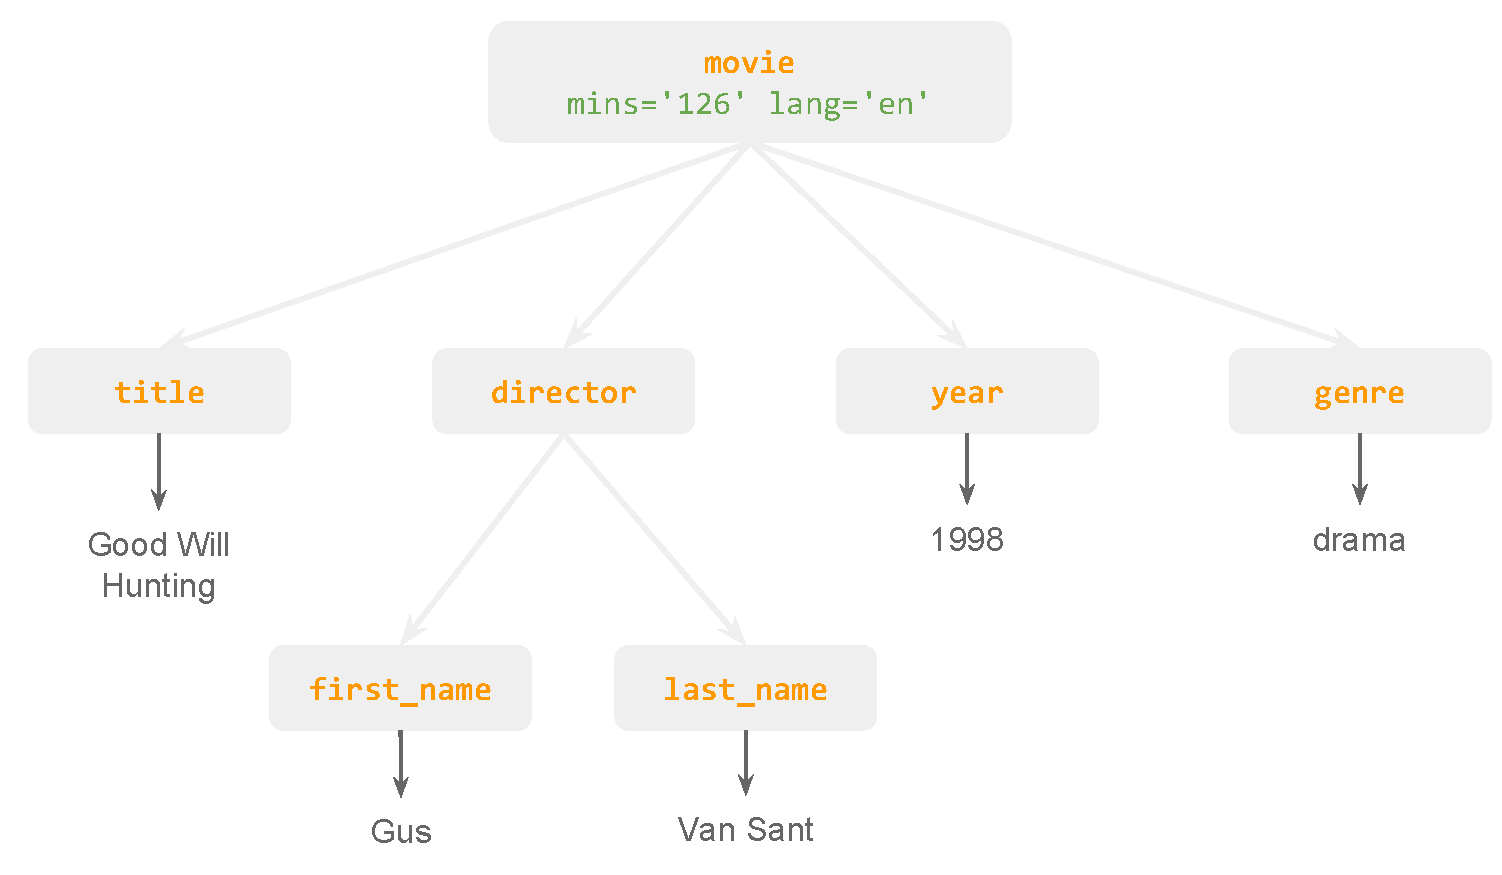
\includegraphics[width=10cm]{xml_movie_tree1.pdf}
\end{center}
\end{frame}

%------------------------------------------------

\begin{frame}
\frametitle{}
\begin{center}
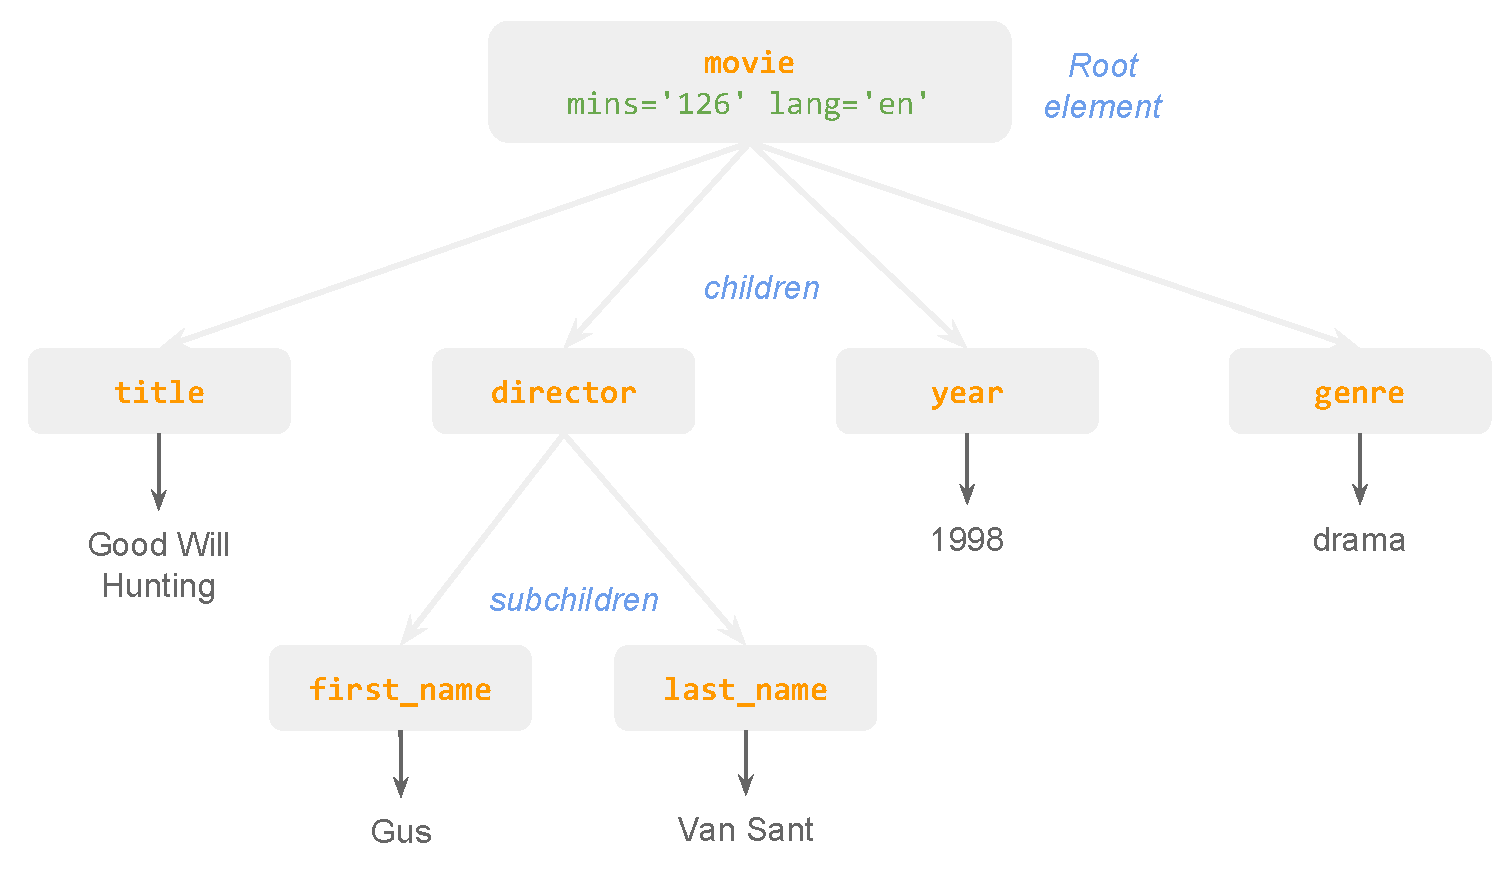
\includegraphics[width=10cm]{xml_movie_tree2.pdf}
\end{center}
\end{frame}

%------------------------------------------------

\begin{frame}
\frametitle{Well-Formedness}

\begin{block}{Well-formed XML}
We say that an XML document is \emph{well-formed} when it obeys the basic syntax rules of XML. Some of those rules are:
\begin{itemize}
 \item One root element containing the rest of elements
 \item Properly nested elements with (self-)closing tags
 \item Attributes appear in start-tags of elements
 \item Attribute values must be quoted
 \item Element names and attribute names are case sensitive
 \item First character for element names must be alphabetic or \_
 \item Values must not contain characters \^~, <, >, \% ~or~ \&
 \item First 3 characters for element names must not be {\it xml}
\end{itemize}
\end{block}

\begin{block}{}
\begin{center}
\emph{Well-formed XML $\neq$ Valid XML}
\end{center}
\end{block}

\end{frame}

%------------------------------------------------

\begin{frame}[fragile]
\frametitle{Well-Formedness}

\begin{verbatim}
<movie mins="126" lang="en">
  <title>Good Will Hunting</title>
  <director>
    <first_name>Gus</first_name>
    <last_name>Van Sant</last_name>
  </director>
  <year>1998</year>
  <genre>drama</genre>
</movie>
\end{verbatim}

\end{frame}

%------------------------------------------------

\begin{frame}
\frametitle{Well-Formedness}

\begin{block}{Importance of Well-formed XML}
Not well-formed XML documents produce potentially fatal errors or warnings when parsed.

\bigskip

Documents may be well-formed but not valid. Well-formed just guarantees that the document meets the basic XML structure, not that the content is valid.
\end{block}

\end{frame}


%------------------------------------------------

\begin{frame}[fragile]
\frametitle{Some Additional Node Types}

{ \small
\begin{verbatim}
<?xml version="1.0"? encoding="UTF-8" ?>
<![CDATA[ a > 5 & b < 10 ]]>
<?GS print(format = TRUE)>
<!DOCTYPE Movie>
<!-- This is a comment -->
<movie mins="126" lang="en">
  <title>Good Will Hunting</title>
  <director>
    <first_name>Gus</first_name>
    <last_name>Van Sant</last_name>
  </director>
  <year>1998</year>
  <genre>drama</genre>
</movie>
\end{verbatim}
}

\end{frame}

%------------------------------------------------

\begin{frame}
\frametitle{Additional Optional XML Elements}

{\small 
\begin{tabular}{l l}
  \hline
  Markup & Description \\
  \hline
  \code{<?xml >} & XML Declaration \\
  & \textit{identifies content as an XML document} \\
  \code{<?PI >} & Processing Instruction \\
  & \textit{processing instructions passed to application} \\
  \code{<!DOCTYPE >} & Document-type Declaration \\
  & \textit{defines the structure of an XML document} \\
  \code{<![CDATA[ ]]>} & CDATA Character Data \\
  & \textit{anything inside a CDATA is ignored by the parser} \\
  \code{<!$--$  $--$>} & Comment \\
  & \textit{for writing comments} \\
  \hline
\end{tabular}
}

\end{frame}

%------------------------------------------------

\begin{frame}
\frametitle{Document-Type Declaration}

\begin{block}{Document-Type Declaration (DTD)}
The Document-type Declaration identifies the \emph{type} of the document. The \textit{type} indicates the structure (i.e., the schema) of a \emph{valid} document: 

\begin{itemize}
 \item What elements are allowed to be present
 \item How elements can be combined
 \item How elements must be ordered
\end{itemize}
\end{block}

~\\
The DTD specifies what the format allows you to do (i.e., semantics), through a language based on regular expressions.

~\\
\begin{block}{}
\emph{XML Schema is the modern alternative to DTD specifications}
\end{block}
\end{frame}



\begin{frame}
\frametitle{XML Schema}

\begin{block}{XML Schema Definition (XSD)}
An XSD is much more specific than a DTD: 

\begin{itemize}
 \item XSD is itself based on XML
 \item Elements are given specific types, such as integer or float 
 \item Elements may be given minimum and maximum values
 \item The XSD may limit the number of times an element may occur
 \item Better support for mixed contents
 \item XSD schemas can use different {\it namespaces}
 \item ...
\end{itemize}
\end{block}

\end{frame}

%------------------------------------------------

\section{XML Namespaces}

\begin{frame}[fragile]{Ambiguity in XML Documents}
\footnotesize
\begin{block}{Ambiguity in XML Documents}
\begin{verbatim}
<table>
    <tr><th>Chairs</th><th>Tables</th></tr>
</table>
<table>
    <wood>cherry</wood>
    <length>48</length>
    <width>18</width>
    <height>12</height>
</table>
\end{verbatim}
\end{block}
\normalsize
\begin{itemize}
	\item An XML file can include both HTML \texttt{<table>} tags and an XML tag for an ordinary table as a piece of furniture.
	\item This structure is ambiguous.
	\item How can this ambiguity be resolved?
\end{itemize}
\end{frame}

\begin{frame}[fragile]{XML Namespaces}
\footnotesize
\begin{block}{XML Namespaces}
\begin{verbatim}
<furniture xmlns:h="http://www.w3.org/TR/html4/"
    xmlns:f="http://www.hsc.edu/myfurniture/">
<h:table><tr><th>Chairs</th><th>Tables</th></tr></h:table>
<f:table>
    <wood>cherry</wood>
    <length>48</length>
    <width>18</width>
    <height>12</height>
</f:table>
\end{verbatim}
\end{block}
\normalsize
\begin{itemize}
	\item Tags may be associated with a \alert{namespace}.
	\item The namespace is a URI (e.g., a Web URL), but its content is not used by the XML processor
	\item Typically, the URI refers to a human-readable web page that explains the meaning of the tags.
\end{itemize}
\end{frame}

\begin{frame}[fragile]{XML Namespaces}
\footnotesize
\begin{block}{XML Namespaces}
\begin{verbatim}
<furniture xmlns:h="http://www.w3.org/TR/html4/"
    xmlns="http://www.hsc.edu/myfurniture/">
<h:table>
    <h:tr><h:th>Chairs</h:th><h:th>Tables</h:th></h:tr>
</h:table>
<table>
    <wood>cherry</wood>
    <length>48</length>
    <width>18</width>
    <height>12</height>
</table>
\end{verbatim}
\end{block}
\normalsize
\begin{itemize}
	\item If the namespace is not given a name, then it is the default namespace.
\end{itemize}
\end{frame}

\section{XPath}

%------------------------------------------------

\begin{frame}[fragile]
\frametitle{XPath}

\begin{block}{Querying Semi-Structured Data in XML}
The real parsing power comes from the ability to \emph{locate nodes and extract information from them}. For this, we need to be able to perform queries on the parsed content.
\end{block}

\begin{block}{XPath}
One solution is provided by \emph{XPath}, which is a language to navigate through elements and attributes in an XML/(X)HTML document.
\end{block}

\end{frame}

%------------------------------------------------

\begin{frame}
\frametitle{XPath}

\begin{block}{XPath}
\begin{itemize}
 \item Is a language for finding information in XML documents
 \item Uses path expressions to select nodes or node-sets in an XML document
 \item Works by identifying patterns to match data or content
 \item Includes hundreds of built-in functions (e.g., for manipulating strings, dates, ...)
 \item Used as part of other technologies for processing XML (e.g., XSLT, XQuery, XML Schema, ...)
\end{itemize}
\end{block}

\end{frame}

%------------------------------------------------

\begin{frame}
\frametitle{About XPath}

\begin{block}{XPath Syntax}
XPath uses \emph{path expressions} to select nodes in an XML document. It has a computational model to identify sets of nodes (node-sets)
\end{block}

\begin{block}{XPath Syntax}
We can specify paths through the tree structure:
\begin{itemize}
 \item Based on node names
 \item Based on node types
 \item Based on node content
 \item Based on a node's relationship to other nodes
\end{itemize}
\end{block}

\end{frame}

%------------------------------------------------

\begin{frame}[fragile]
\frametitle{About XPath}

\begin{block}{XPath Syntax}
The key concept is knowing how to write path expressions.

~\\

XPath expressions have a syntax similar to the way files are located in a hierarchy of directories/folders in a computer file system. For instance


\bigskip 
\begin{center}
\code{/movies/movie[1]}
\end{center}
\bigskip
is the XPath expression to locate the first {\hilit \code{movie}} element that is the child of the {\hilit \code{movies}} element
\end{block}
\end{frame}

%------------------------------------------------

\begin{frame}
\frametitle{Selecting Nodes}

\begin{block}{XPath Abbreviated Syntax}
The main path expressions (i.e., symbols) are:
\end{block}

\begin{center}
 \begin{tabular}{l l}
  \hline
  Symbol & Description \\
  \hline
  \code{/} & Selects childs from the context node \\
  \code{//} & Selects desdendant nodes anywhere \\
  \code{.} & Selects the current node \\
  \code{..} & Selects the parent of the current node \\
  \code{@} & Selects attributes \\
  \code{[]} & Square brackets to indicate predicates \\
  \hline
 \end{tabular}
\end{center}

\end{frame}

%------------------------------------------------

\begin{frame}
\frametitle{XPath Predicates}
XPath predicates (square brackets \code{[]}) allow you to find a specific node or node\(s\) that contains a specific value.

~\\

You can use the usual comparison operators <, <=, etc.  A major difference is that equality is = and \textbf{NOT} ==.  

~\\

An example usage might be:

\begin{center}
\code{/store//plants/flowers[@avgheight>10]}
\end{center}

This would search on descendants from the \emph{store} element for flowers with an \emph{attribute} \emph{avgheight} greater than 10.
\end{frame}

\begin{frame}[fragile]{XPath Axes}
\begin{itemize}
	\item The full syntax for XPath supports navigation over multiple \alert{axes}
	\item Examples are \texttt{.} and \texttt{..}
	\item The following axes are available.
	\begin{itemize}
		\item \texttt{self} or ``\texttt{.}''
		\item \texttt{child} or ``\texttt{/}'' (i.e., default axis)
		\item \texttt{parent} or ``\texttt{..}''
		\item \texttt{descendant} or ``\texttt{//}''
		\item \texttt{ancestor}
		\item \texttt{preceding-sibling}
		\item \texttt{following-sibling}
	\end{itemize}
	\item The axis is always relative to the context node.
\end{itemize}
\end{frame}

\begin{frame}[fragile]{XPath Axes}
\small
\begin{block}{XPath Axes}
\begin{semiverbatim}
\textit{axis-name}::\textit{node-name}[\textit{predicate}]
\end{semiverbatim}
\end{block}
\normalsize
\begin{itemize}
	\item The axis name is followed by \texttt{::}
	\item The default axis is \texttt{child::}
\end{itemize}
\end{frame}

%------------------------------------------------

\begin{frame}
\frametitle{Selecting Unknown Nodes}

\begin{block}{XPath wildcards for unknown nodes}
XPath wildcards can be used to select unknown XML elements
\end{block}

\begin{center}
 \begin{tabular}{l l}
  \hline
  Symbol & Description \\
  \hline
  \code{*} & matches any element node \\
  \code{@*} & matches any attribute node \\
  \code{node()} & matches any node of any kind \\
  \code{element()} & matches any element \\
  \code{text()} & matches any textual content node \\
  \hline
 \end{tabular}
\end{center}

\end{frame}

\begin{frame}[fragile]{XPath Functions}
\begin{itemize}
	\item XPath provides a number of functions.
	\begin{itemize}
		\item \texttt{data()}
		\item \texttt{count()}
		\item \texttt{sum()}
		\item \texttt{avg()}
		\item \texttt{min()}
		\item \texttt{max()}
		\item \texttt{contains()}
		\item \texttt{starts-with()}
	\end{itemize}
	\item See
	\small \url{https://www.w3schools.com/xml/xsl_functions.asp} \normalsize for a complete list of XPath functions.
\end{itemize}
\end{frame}

%------------------------------------------------

\begin{frame}
\frametitle{Movies Tree Structure}
\begin{center}
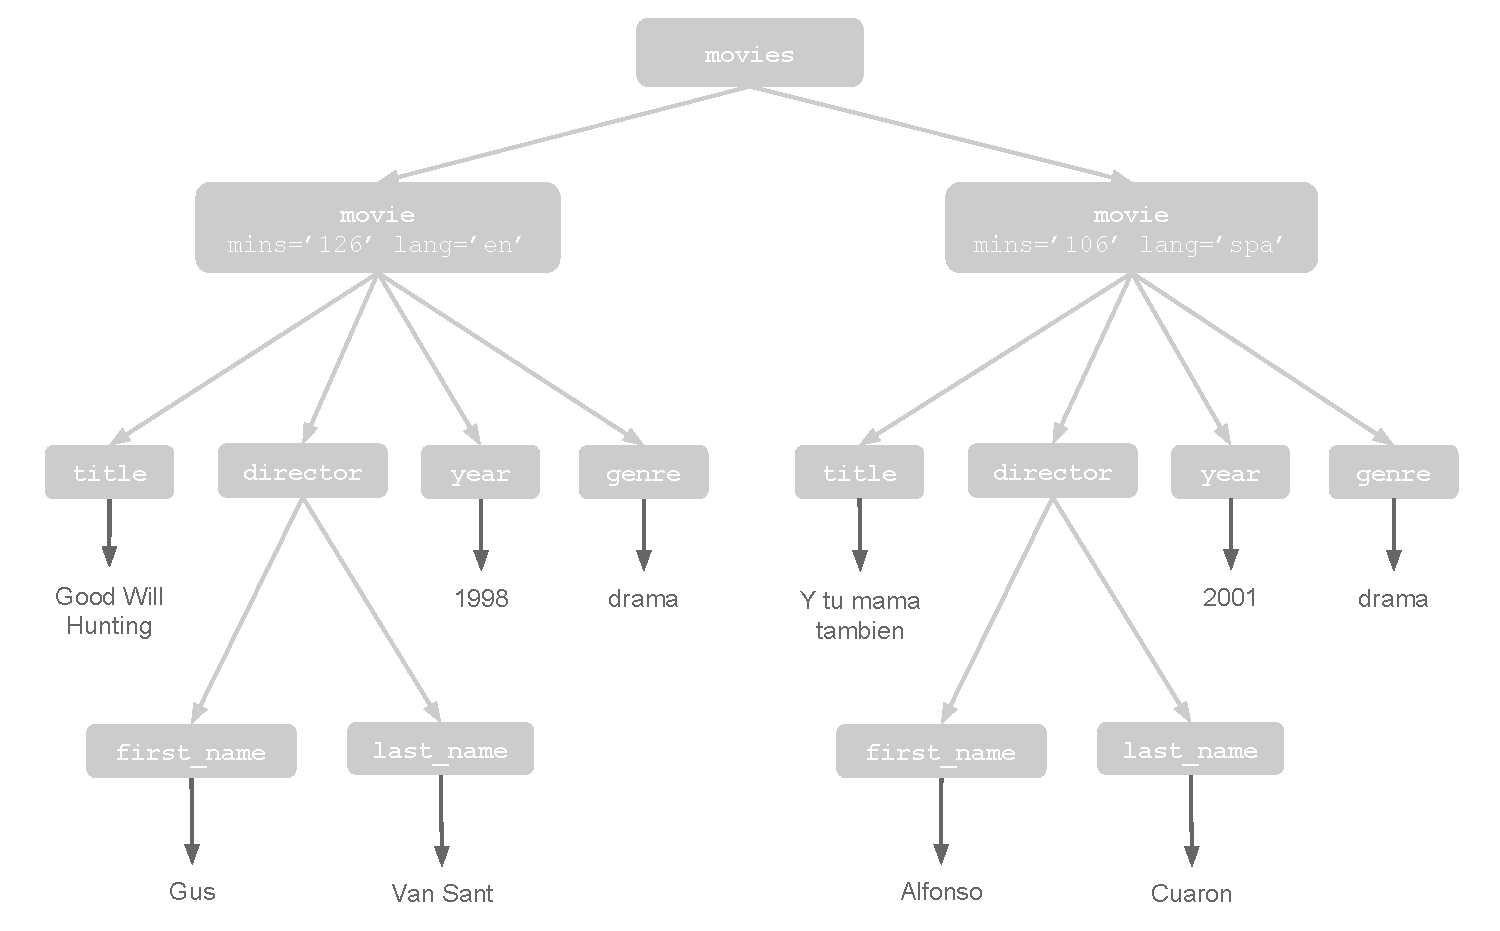
\includegraphics[width=10cm]{xpath_tree.pdf}
\end{center}
\end{frame}

%------------------------------------------------

\begin{frame}
\frametitle{XPath: movie nodes}
\begin{center}
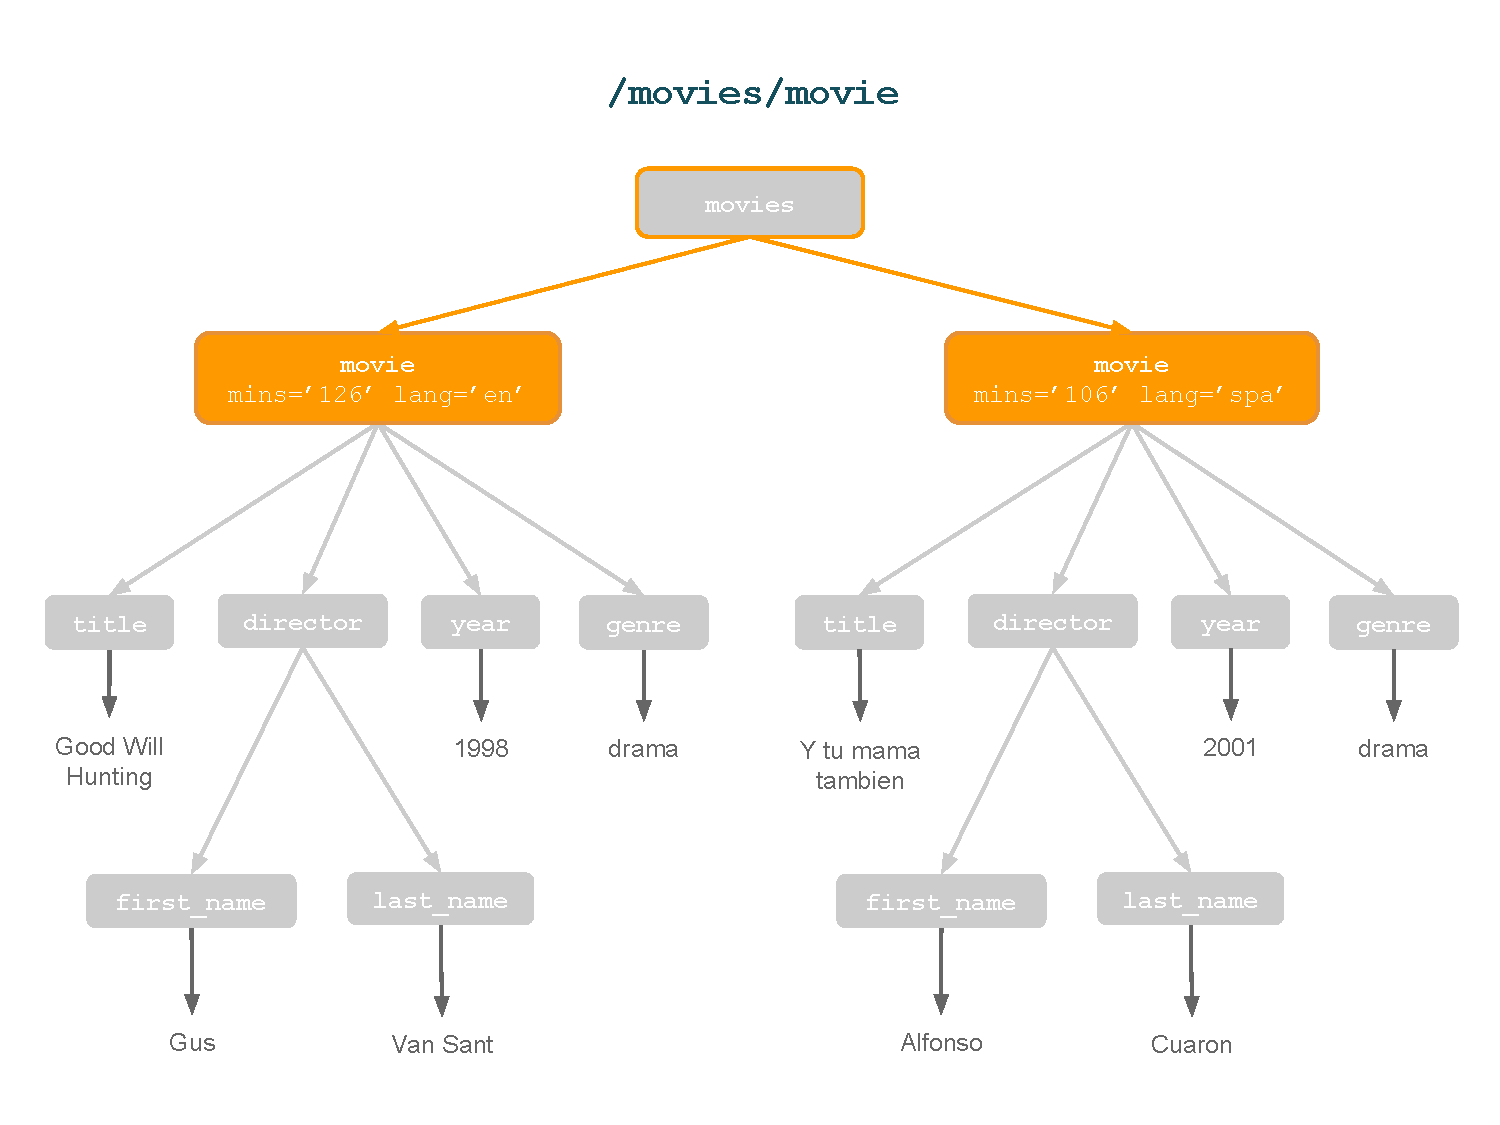
\includegraphics[width=10cm]{xpath_movie.pdf}
\end{center}
\end{frame}

%------------------------------------------------

\begin{frame}
\frametitle{XPath: movie title nodes}
\begin{center}
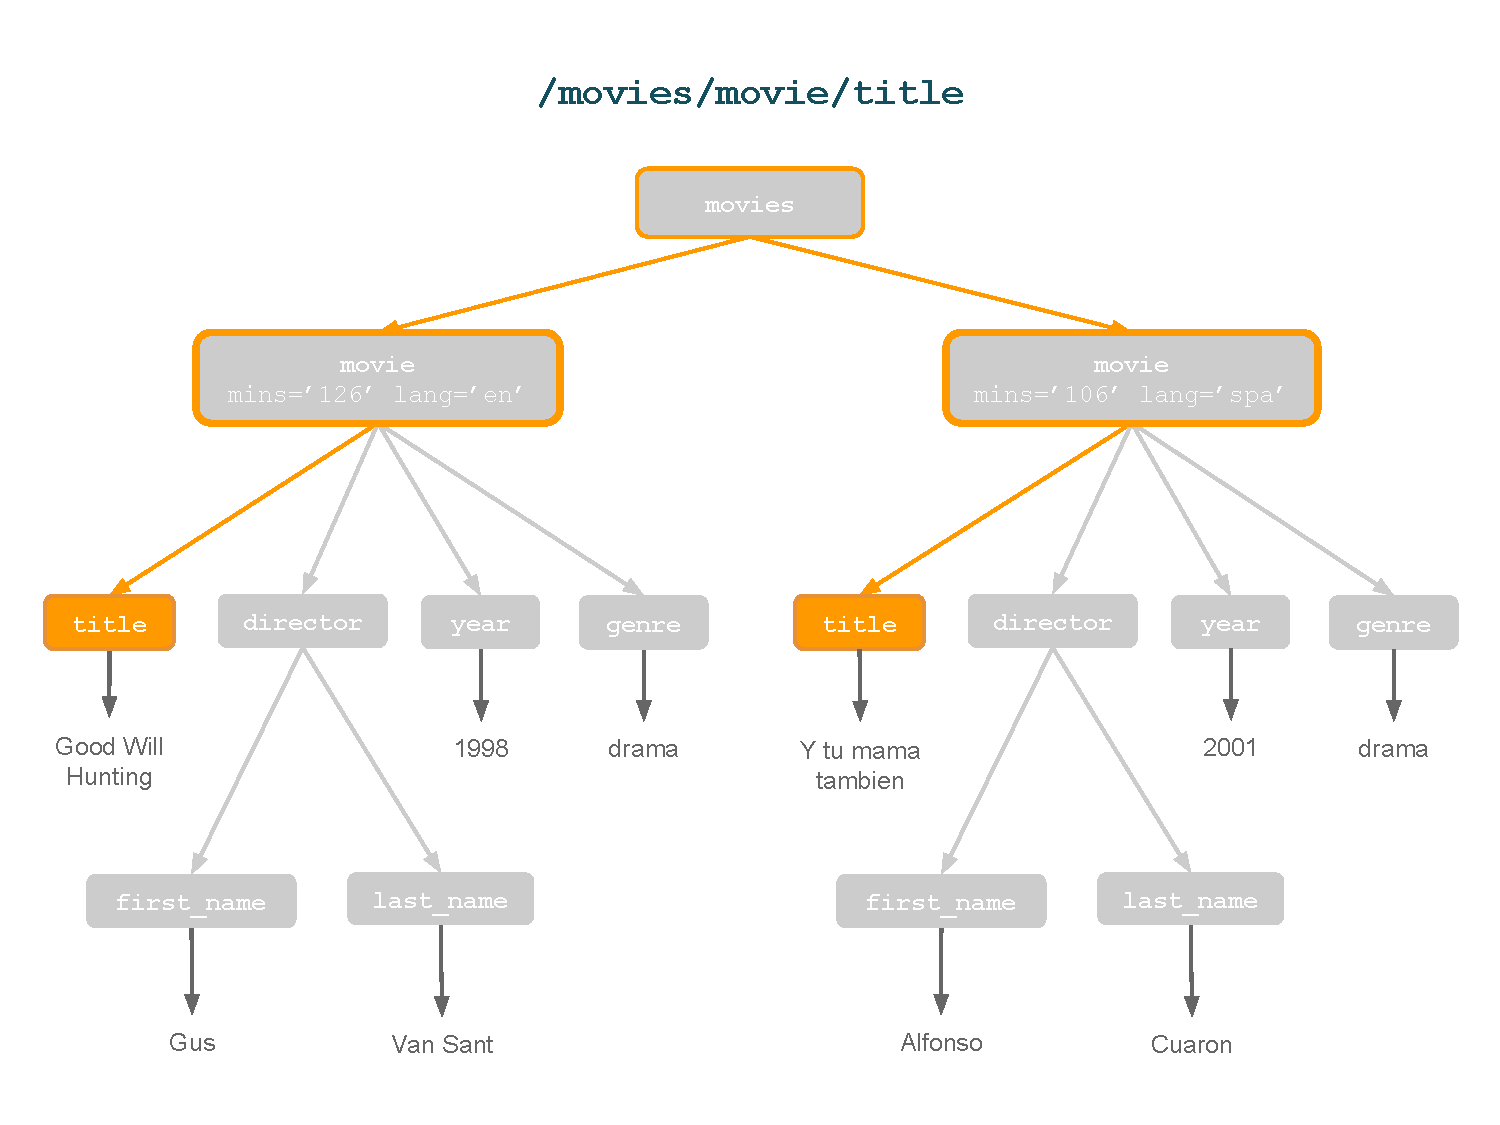
\includegraphics[width=10cm]{xpath_title.pdf}
\end{center}
\end{frame}

%------------------------------------------------

\begin{frame}
\frametitle{XPath: movie director's first name nodes}
\begin{center}
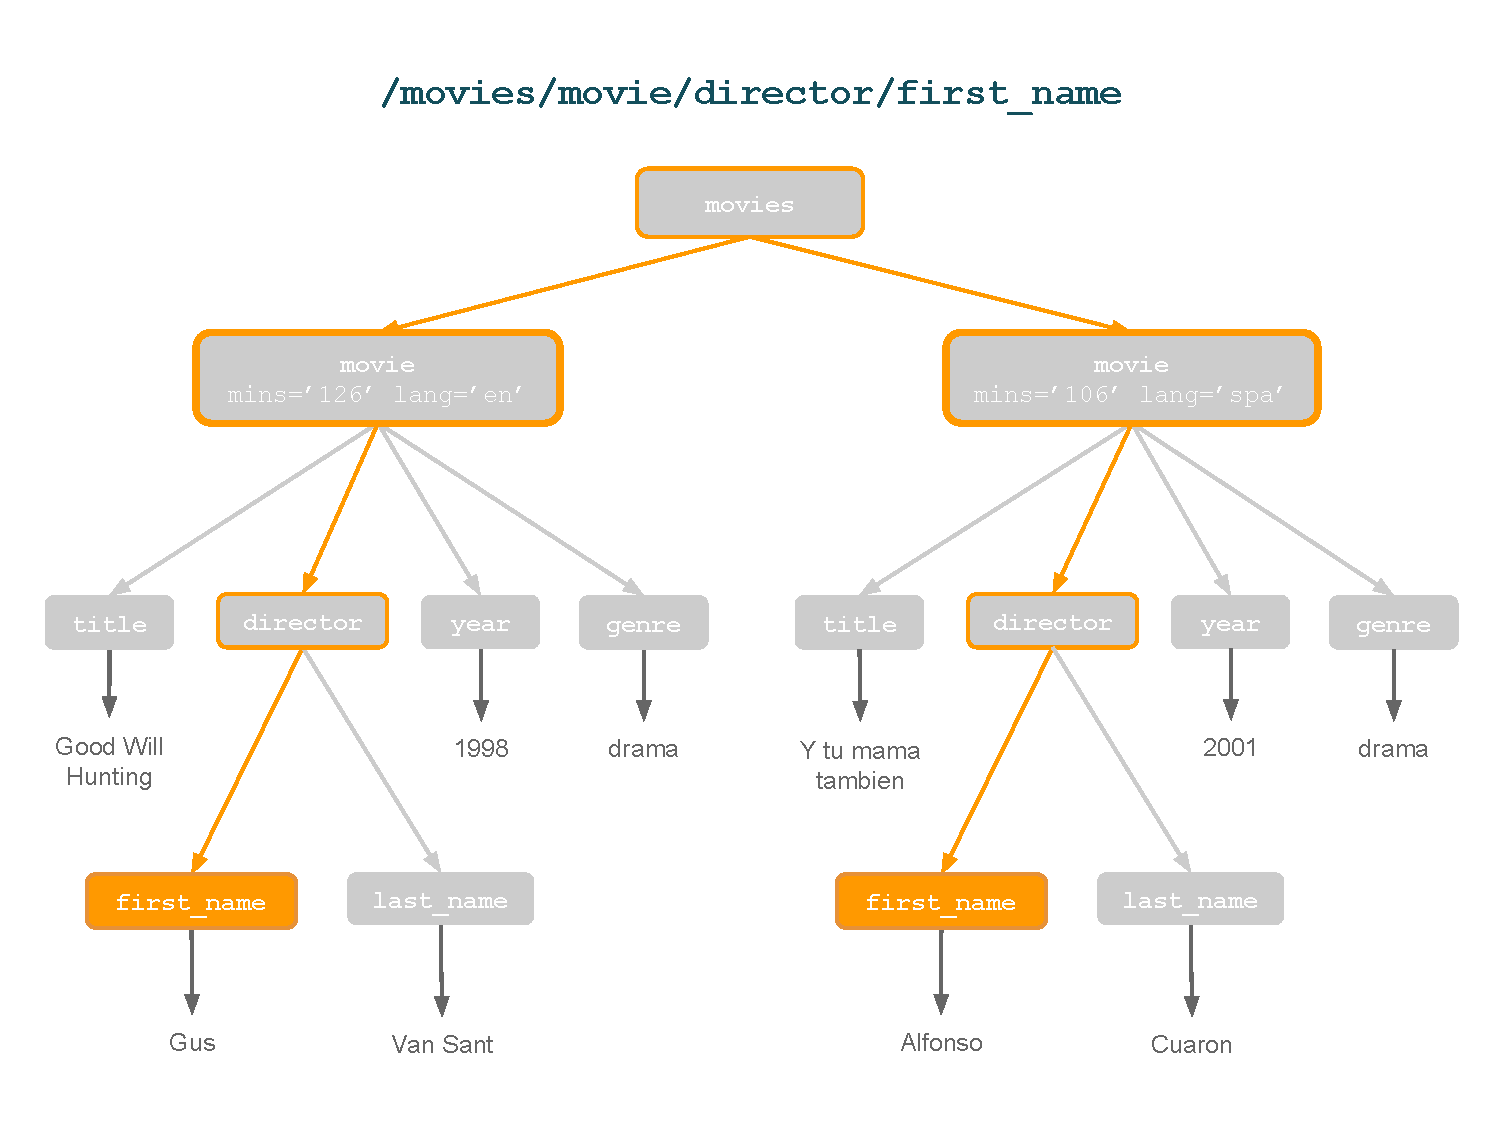
\includegraphics[width=10cm]{xpath_firstname.pdf}
\end{center}
\end{frame}

%------------------------------------------------

\begin{frame}
\frametitle{XPath: movie director nodes}
\begin{center}
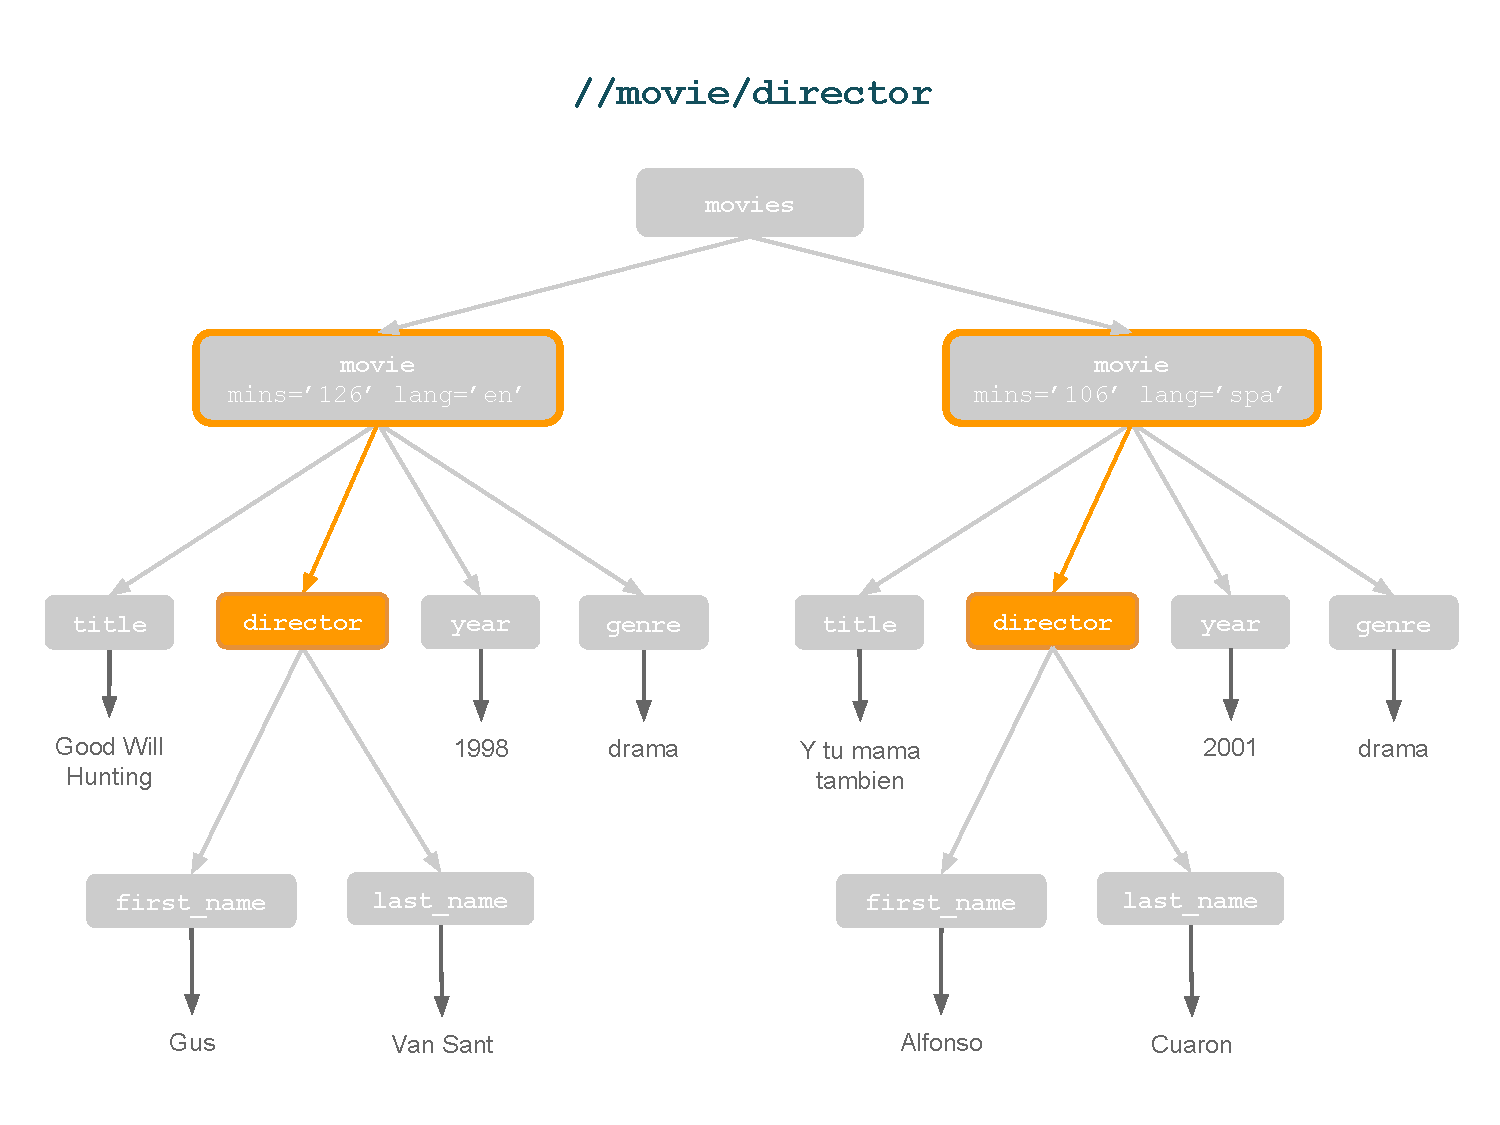
\includegraphics[width=10cm]{xpath_director.pdf}
\end{center}
\end{frame}

%------------------------------------------------

\begin{frame}
\frametitle{XPath: last name nodes}
\begin{center}
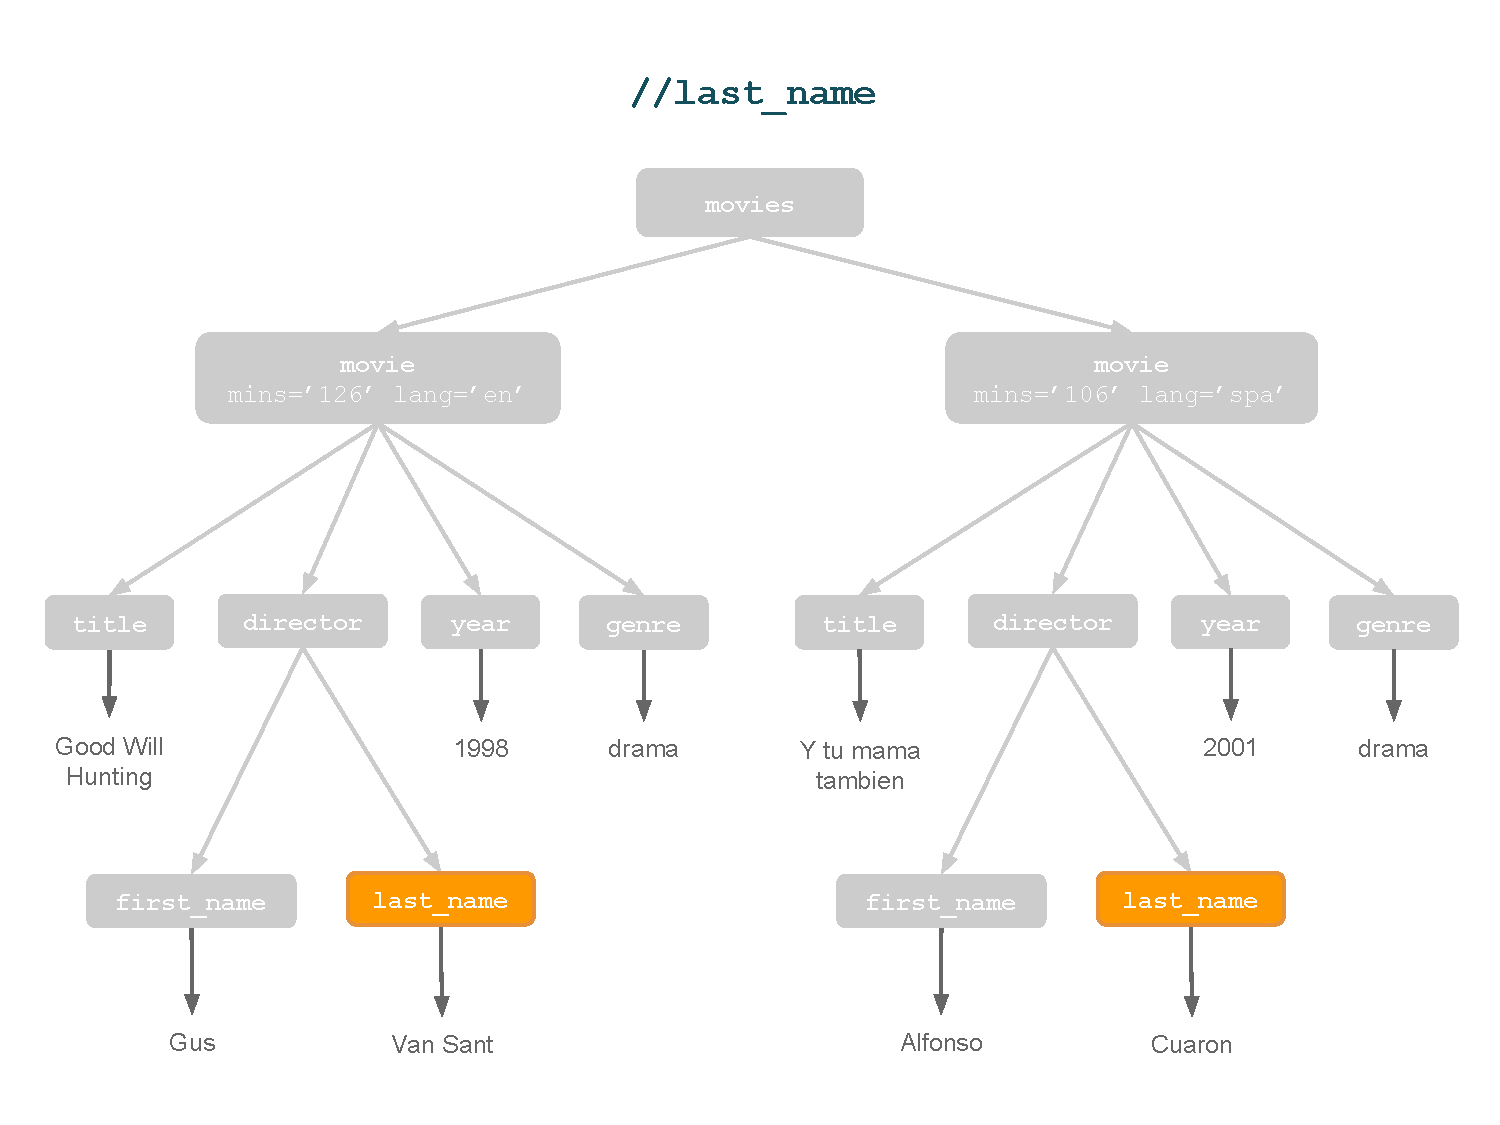
\includegraphics[width=10cm]{xpath_lastname.pdf}
\end{center}
\end{frame}

%------------------------------------------------

\begin{frame}
\frametitle{XPath: title node of movie in Spanish}
\begin{center}
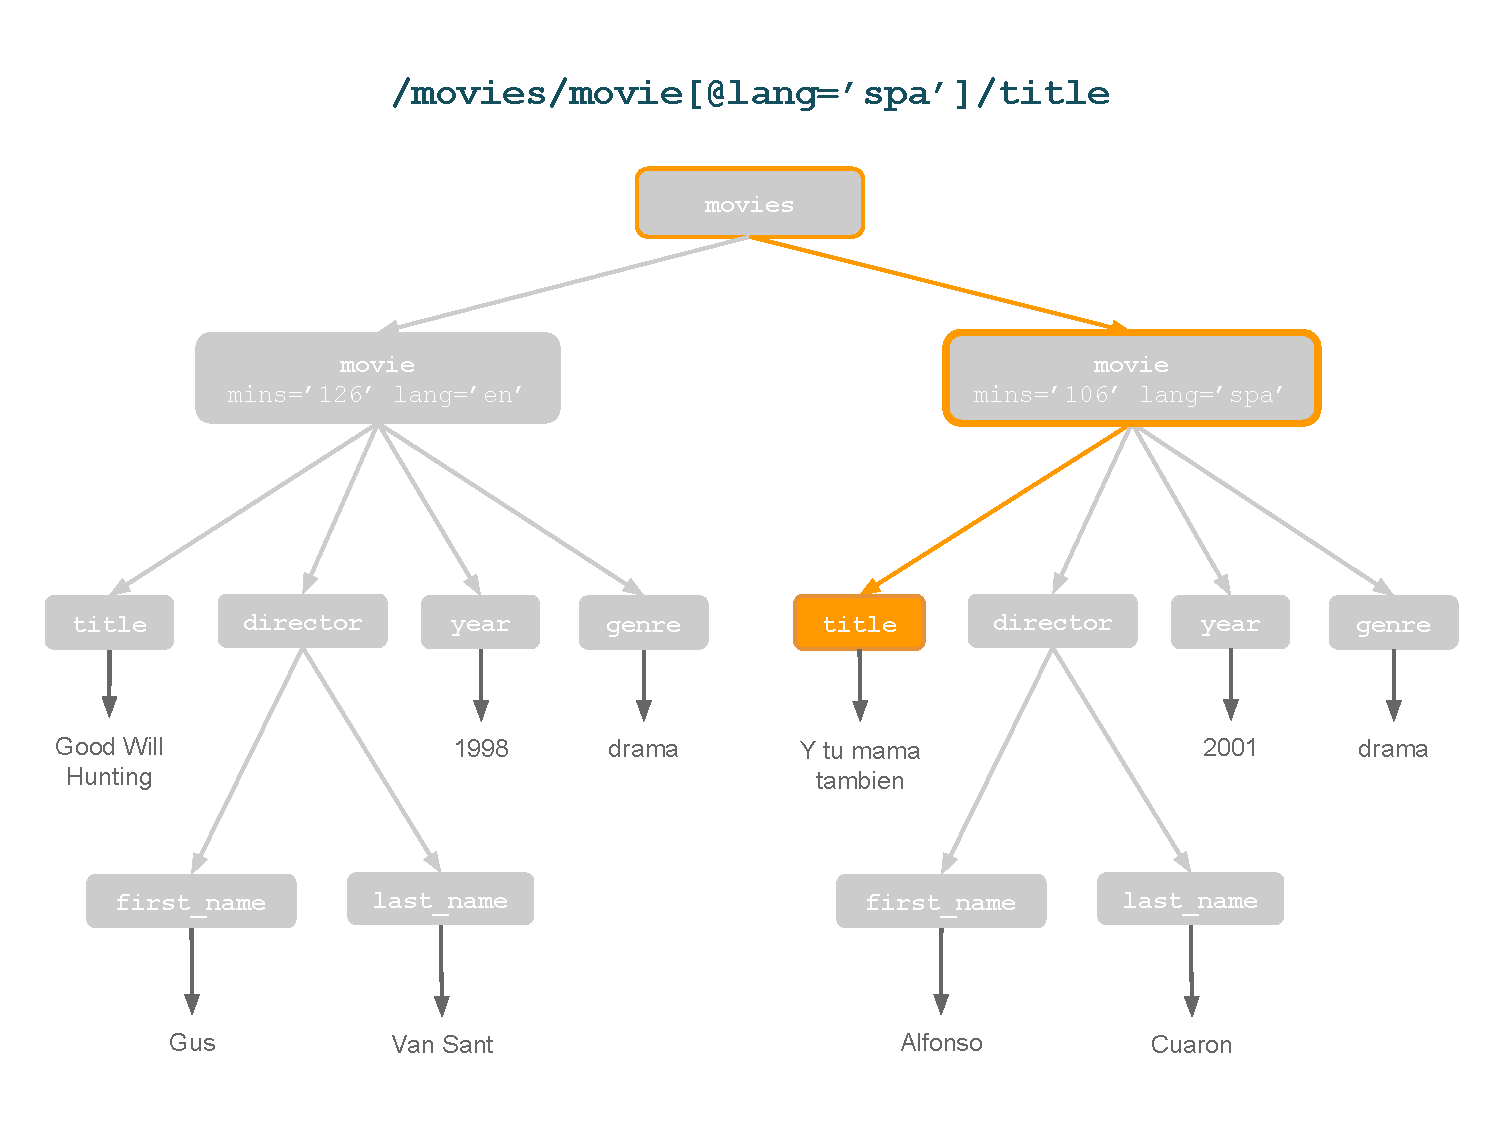
\includegraphics[width=10cm]{xpath_ytmt.pdf}
\end{center}
\end{frame}

\section{(X)HTML}

\begin{frame}[fragile]{HTML}
\begin{itemize}
	\item HTML = Hypertext Markup Language.
	\item Recall that {\it markup} refers to \alert{tags} embedded within the text that tell how the text is to be rendered.
	\item For example, the \texttt{<b>} tag will render text in boldface.
	\item \emph{Hypertext} refers to links to other documents or links within the same document.
	\item The anchor tag \texttt{<a>} contains a \text{hyperreference}.
\end{itemize}
\end{frame}

\begin{frame}[fragile]{HTML Tags}
\begin{itemize}
	\item Most tags have a corresponding closing tag.
	\item For example, the closing tag for \texttt{<b>} is \texttt{</b>}.
	\item A few tags are self-closing.
	\item For example, the line break tag \texttt{<br/>} is self-closing.
\end{itemize}
\end{frame}

\begin{frame}[fragile]{HTML Structure}
\small
\begin{block}{HTML Structure}
\begin{semiverbatim}
<html>
    <head>
        \emph{headers}
    </head>
    <body>
        \emph{body of document}
    </body>
</html>
\end{semiverbatim}
\end{block}
\normalsize
\begin{itemize}
	\item An HTML document is enclosed in \texttt{<html>} tags.
	\item Within these tags are the \texttt{<head>} and \texttt{<body>} sections.
\end{itemize}
\end{frame}

\begin{frame}[fragile]{The Header}
\small
\begin{block}{Titles}
\begin{verbatim}
<head>
    <title>My First Webpage</title>
</head>
\end{verbatim}
\end{block}
\normalsize
\begin{itemize}
	\item The header may contain the title of the page.
	\item The title will appear in the title bar of the browser window.
	\item The header section typically also contains descriptive meta-tags (e.g., key-words).
	\item An XPath expression like {\tt /html/head/title/text()} would retrieve the title for the HTML document.
\end{itemize}
\end{frame}

\begin{frame}[fragile]{The Body}
\small
\begin{block}{Paragraphs}
\begin{verbatim}
<body>
    <p>This is the first paragraph.

    This is still the first paragraph.</p>
    <p>This is the second paragraph.</p>
</body>
\end{verbatim}
\end{block}
\normalsize
\begin{itemize}
	\item The body contains the content to be displayed.
	\item Text that is not within tags is rendered as plain text.
	\item Every span of white space characters is equivalent to a single blank space when rendering the content.
	\item The paragraph tag \texttt{<p>} can be used to break the content into paragraphs.
\end{itemize}
\end{frame}

\begin{frame}[fragile]{Basic Example}
\begin{block}{Basic Example}
\small
\begin{verbatim}
<html>
<head>
<title>My First Web Page</title>
</head>
<body>
<p>Q: Why did the chicken cross the road?</p>
<p>A: To prove to the opossum that it could be done.</p>
</body>
</html>
\end{verbatim}
\normalsize
\end{block}
\end{frame}

\begin{frame}[fragile]{Headings}
\small
\begin{block}{Headings}
\begin{verbatim}
<h1>Bruno Emanuel Martins</h1>
<h2>Information Processing and Retrieval</h2>
<h3>MEIC/METI - IST</h3>
<h4>Fall Semester</h4>
<h5>Theoretical Lecture: Semi-Structured Data</h5>
<h6>09h30</h6>
\end{verbatim}
\end{block}
\normalsize
\begin{itemize}
	\item Six levels of headings, with tags \texttt{<h1>} through \texttt{<h6>}.
	\item Level 1 is the largest; level 6 is the smallest.
\end{itemize}
\end{frame}

\begin{frame}[fragile]{Headings}
\small
\begin{block}{Centering}
\scriptsize
\begin{verbatim}
<h1 align="center">Bruno Emanuel Martins</h1>
<h2 align="center">Information Processing and Retrieval</h2>
<h3 align="center">MEIC/METI - IST</h3>
<center>
 <h4>Fall Semester</h4>
 <h5>Theoretical Lecture: Semi-Structured Data</h5>
 <h6>09h30</h6>
</center>
\end{verbatim}
\end{block}
\normalsize
\begin{itemize}
	\item The headings may be centered.
	\begin{itemize}
		\item Use the \texttt{<center>} tag, or
		\item Use the \texttt{align} \alert{attribute}.
	\end{itemize}
\end{itemize}
\end{frame}

\begin{frame}[fragile]{Text Face}
\begin{itemize}
	\item There are several choices for the text face.
	\begin{itemize}
		\item \texttt{<b>}\textbf{Bold text}\texttt{</b>}
		\item \texttt{<i>}{\it Italic text}\texttt{</i>}
		\item \texttt{<tt>}\texttt{Teletype text}\texttt{</tt>}
	\end{itemize}
	\item Combinations are possible.
	\begin{itemize}
		\item \texttt{<b><i>}\textbf{\textit{Bold Italic text}}\texttt{</i></b>}
		\item \texttt{<i><tt><b>}{\it \textbf{\texttt{Italic Teletype Bold}}}\texttt{</b></tt></i>}
	\end{itemize}
\end{itemize}
\end{frame}

\begin{frame}[fragile]{Lists}
\begin{itemize}
	\item We can use ordered lists \texttt{<ol>} or unordered lists \texttt{<ul>}.
	\item An unordered list is a bulleted list.
	\item An ordered list is a numbered list.
	\item Each item in a list is tagged with a list-item tag \texttt{<li>}.
\end{itemize}
\end{frame}

\begin{frame}[fragile]{Lists}
\small
\begin{block}{Unordered List}
\begin{verbatim}
<ul>
    <li>Instituto Superior Técnico</li>
    <li>Faculdade de Ciências</li>
    <li>Faculdade de Medicina</li>
    <li>Faculdade de Letras</li>
</ul>
\end{verbatim}
\end{block}
\normalsize
\begin{itemize}
	\item An unordered list of schools.
\end{itemize}
\end{frame}

\begin{frame}[fragile]{Lists}
\small
\begin{block}{Ordered List}
\begin{verbatim}
<ol>
    <li>Instituto Superior Técnico</li>
    <li>Faculdade de Ciências</li>
    <li>Faculdade de Medicina</li>
    <li>Faculdade de Letras</li>
</ol>
\end{verbatim}
\end{block}
\normalsize
\begin{itemize}
	\item An ordered list of schools.
\end{itemize}
\end{frame}

\begin{frame}[fragile]{Hyperreferences}
\small
\begin{block}{Hyperreference}
\begin{semiverbatim}
<a href='\emph{hyperreference}'>\textit{link\_text}</a>
\end{semiverbatim}
\end{block}
\normalsize
\begin{itemize}
	\item An anchor tag \texttt{<a>} is used to create a hyperreference.
	\item When the user clicks on the \texttt{\textit{link\_text}}, the link is activated.
\end{itemize}
\end{frame}

\begin{frame}[fragile]{Hyperreferences}
\scriptsize
\begin{block}{Hyperreference}
\begin{verbatim}
Look at us <a href="https://tecnico.ulisboa.pt/">here</a>
\end{verbatim}
\end{block}
\normalsize
\begin{itemize}
	\item Usually, the link text will appear underlined and in a different color.
\end{itemize}
\end{frame}

\begin{frame}[fragile]{Images}
\small
\begin{block}{Images}
\begin{semiverbatim}
<img src="\emph{filename or URL}" />
\end{semiverbatim}
\end{block}
\normalsize
\begin{itemize}
	\item An image may be included in a document by using the image tag \texttt{<img>}.
	\item An \texttt{alt} attribute may be included, in case the image does not load.
	\item The height and width of the displayed image may be included, using the \texttt{height} and \texttt{width} attributes.
\end{itemize}
\end{frame}

\begin{frame}[fragile]{Images}
\scriptsize
\begin{block}{Images}
\begin{verbatim}
Course instructor: 
<img src="http://bgmartins.github.io/my-photo.jpg" 
	alt="Bruno Martins" height="314" width="336" />
\end{verbatim}
\end{block}
\normalsize
\begin{itemize}
	\item The height and width do not need to match the dimensions of the image.
\end{itemize}
\end{frame}

\begin{frame}[fragile]{Tables}
\begin{itemize}
	\item The table tag \texttt{<table>} may be used to format information in tabular form.
	\item Within the table element we may list any number of table rows, using the \texttt{<tr>} tag.
	\item Each entry in a row is indicated by a table data tag \texttt{<td>} within the table row elements.
\end{itemize}
\end{frame}

\begin{frame}[fragile]{Tables}
\small
\begin{block}{Tables}
\begin{semiverbatim}
<table>
    <tr>
        <td>\textit{table\_entry}</td>
            \vdots
        <td>\textit{table\_entry}</td>
    </tr>
        \vdots
</table>
\end{semiverbatim}
\end{block}
\end{frame}

\begin{frame}[fragile]{Tables}
\small
\begin{block}{Tables}
\begin{semiverbatim}
<table>
    <tr>
        <th>\textit{column\_heading}</th>
            \vdots
        <th>\textit{column\_heading}</th>
    </tr>
        \vdots
</table>
\end{semiverbatim}
\end{block}
\normalsize
\begin{itemize}
	\item The first row (or any row) of a table may be designated as table headings by using the \texttt{<th>} tag instead of the \texttt{<td>} tags.
\end{itemize}
\end{frame}

\begin{frame}{Tables}
\begin{itemize}
	\item The \texttt{<table>} tag may take a number of attributes.
	\begin{itemize}
		\item \texttt{border} = Size of the table border, in pixels.
		\item \texttt{cellpadding} = Padding within cells between the table entry and the cell border, in pixels.
		\item \texttt{cellspacing} = Spacing between adjacent cell borders, in pixels.
		\item \texttt{width} = Width of the table either in pixels or as a percent of the window's width.
	\end{itemize}
\end{itemize}
\end{frame}

\begin{frame}{Tables}
\begin{center}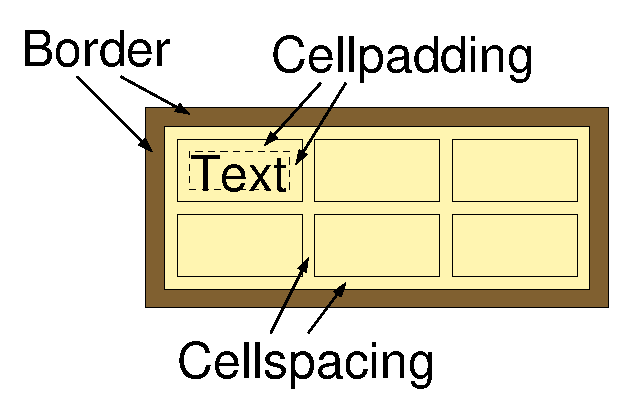
\includegraphics[scale=0.60]{Fig-1.pdf}\end{center}
\end{frame}

% ------------------------------------------------------------

\finalframe{Questions?}

\end{document}
 